\section{Physikalische Grundlagen der Wärmestrahlung}
Zum Verständnis des Treibhauseffekts ist es essenziell zu untersuchen, wie die Erde den Großteil ihrer Energie erhält und 
wie sie ihre überschüssige Energie wieder abgibt. Der Energiehaushalt der Erde wird hauptsächlich durch 
Strahlungsprozesse bestimmt: Die Erde erhält Energie durch Strahlung der Sonne und strahlt selbst wieder Energie in
den Weltraum \cite[S.~9--11]{marshall2007atmosphere}. Im folgenden Kapitel werden diese Strahlungsprozesse im Detail betrachtet, um die Grundlage
des Treibhauseffekts zu verstehen.

\subsection{Grundbegriffe der elektromagnetischen Strahlung}
\textit{Wärmestrahlung} bezeichnet die elektromagnetische Strahlung, die von Materie aufgrund ihrer thermischen
Energie emittiert wird. Elektromagnetische Strahlung ist eine Form der Energieübertragung, die sich im Raum ausbreitet und entweder 
als elektromagnetische Wellen (wie von der elektromagnetischen Wellentheorie beschrieben; \cite{electricityMagnetism})
oder als masselose Energiequanten, sogenannte \textit{Photonen} (wie von der Quantenmechanik beschrieben; \cite{quantumMechanics}),
aufgefasst werden kann. Keine der beiden Sichtweisen kann alle beobachteten Strahlungsphänomene vollständig beschreiben, weshalb beide
Konzepte komplementär verwendet werden. \cite[S.~1--2]{radiativeHeatTransfer}

Elektromagnetische Strahlung bewegt sich mit der \textit{Lichtgeschwindigkeit} $c = c_0/n$, wobei $c_0 = \SI{2.998e8}{\meter\per\second}$ 
die Lichtgeschwindigkeit im Vakuum ist und $n$ den Brechungsindex des Mediums bezeichnet. 
Da die in dieser Arbeit betrachteten Strahlungsprozesse hauptsächlich im Vakuum ($n \equiv 1$) oder 
in Luft ($n \approx 1.0002$) stattfinden, wird im Folgenden die Näherung $n = 1$ und somit $c = c_0$ verwendet \cite[S.~3]{radiativeHeatTransfer}.
Das elektromagnetische Spektrum wird nach der Wellenlänge in verschiedene Bereiche unterteilt, wobei für die Wärmeübertragung insbesondere die 
ultraviolette Strahlung (UV, $\lambda < \SI{380}{\nano\meter}$), das sichtbare Licht ($\SI{380}{\nano\meter} \leq \lambda \leq \SI{780}{\nano\meter}$) 
und die infrarote Strahlung (IR, $\lambda > \SI{780}{\nano\meter}$) von Bedeutung sind. Elektromagnetische Wellen werden durch folgende Eigenschaften charakterisiert:
\begin{table}[H]
    \centering
    \small
    \begin{tabularx}{1\textwidth}{l X}
        \toprule
        \textbf{Eigenschaft} & \textbf{Beschreibung und Einheit} \\
        \midrule
        Frequenz, $\nu$ & Anzahl der Schwingungen pro Zeiteinheit, $[\si{\hertz}] = [\si{\second}^{-1}]$ \\
        Wellenlänge, $\lambda$ & Abstand zwischen zwei Wellenmaxima, $[\si{\micro\meter}]$ oder $[\si{\nano\meter}]$ \\
        Wellenzahl, $\eta$ & Anzahl der Wellen pro Längeneinheit, $[\si{\centi\meter}^{-1}]$ \\
        \bottomrule
    \end{tabularx}
    \caption{Charakteristische Eigenschaften elektromagnetischer Wellen \cite[S.~4]{radiativeHeatTransfer}.}
    \label{tab:wave_properties}
\end{table}
\vspace{-0.5cm} 
\ifthenelse{\boolean{formeln}}{
  \begin{equation}
    \nu = \frac{c_0}{\lambda} = c_0\eta
    \quad \text{\cite[S.~4]{radiativeHeatTransfer}}
  \end{equation}
}{}
\ifthenelse{\boolean{abbildungen}}{
  \begin{figure}[H]
  \centering
  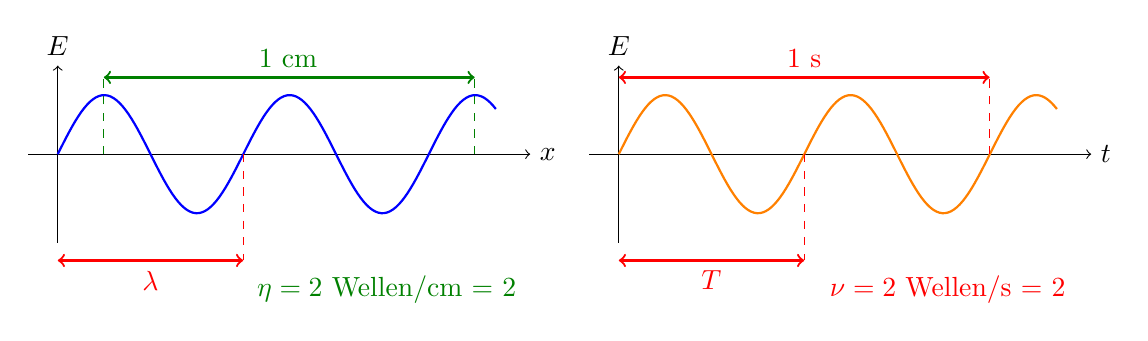
\begin{tikzpicture}[scale=0.75]
      \begin{scope}[xshift=0cm]
          \draw[->] (-0.5,0) -- (8,0) node[right] {$x$};
          \draw[->] (0,-1.5) -- (0,1.5) node[above] {$E$};
          \draw[thick, blue] plot[domain=0:7.42, samples=150] (\x, {sin(2*\x r)});
          
          \draw[<->, red, thick] (0,-1.8) -- (3.14,-1.8) node[midway, below] {$\lambda$};
          \draw[red, dashed] (3.14,0) -- (3.14,-1.8);
          
          \draw[<->, green!50!black, thick] (0.78,1.3) -- (7.06,1.3);
          \node[green!50!black, above] at (3.9,1.3) {1 cm};
          
          \draw[green!50!black, dashed] (0.78,0) -- (0.78,1.3);
          \draw[green!50!black, dashed] (7.06,0) -- (7.06,1.3);
          \node[green!50!black] at (5.57,-2.3) {$\eta = 2$ Wellen/cm = \SI{2}{\per\centi\meter}};
      \end{scope}
      
      \begin{scope}[xshift=9.5cm]
          \draw[->] (-0.5,0) -- (8,0) node[right] {$t$};
          \draw[->] (0,-1.5) -- (0,1.5) node[above] {$E$};
          \draw[thick, orange] plot[domain=0:7.42, samples=150] (\x, {sin(2*\x r)});
          
          \draw[<->, red, thick] (0,1.3) -- (6.28,1.3);
          \node[red, above] at (3.14,1.3) {1 s};
          \draw[red, dashed] (6.28,0) -- (6.28,1.3);

          \draw[<->, red, thick] (0,-1.8) -- (3.14,-1.8) node[midway, below] {$T$};
          \draw[red, dashed] (3.14,0) -- (3.14,-1.8);


          \node[red] at (5.57,-2.3) {$\nu = 2$ Wellen/s = \SI{2}{\hertz}};
      \end{scope}
  \end{tikzpicture}
  \caption{Visualisierung charakteristischer Eigenschaften elektromagnetischer Wellen. 
  Links: Räumliche Darstellung zeigt die Wellenlänge $\lambda$ und die Wellenzahl $\eta$. 
  Rechts: Zeitliche Darstellung zeigt die Periode $T$ und die Frequenz $\nu$.}
  \label{fig:wave_space_time}
  \end{figure}
}{}

\subsection{Strahlungsgesetze}
\label{sec:strahlungsgesetzte}
Jedes Medium emittiert elektromagnetische Strahlung isotrop in alle Richtungen. 
Die Intensität dieser Emission hängt sowohl von der Temperatur als auch von den Materialeigenschaften des Mediums ab. 
Der von einer Oberfläche abgegebene Strahlungswärmestrom wird als \textit{spezifische Ausstrahlung} $E$ bezeichnet und quantifiziert die Intensität der Emission.

Dabei wird zwischen der \textit{gesamten spezifischen Ausstrahlung} $E$ und der \textit{spektralen spezifischen Ausstrahlung} $E_{\nu}$ unterschieden:
\ifthenelse{\boolean{formeln}}{
  \begin{align*}
  E_{\nu} &\equiv \text{abgestrahlte Energie pro Zeit, Oberfläche und Frequenz (spektrale Intensität).} \\
  E &\equiv \text{abgestrahlte Energie pro Zeit und Oberfläche (Gesamtintensität).}
  \end{align*}
}{}
\cite[S.~6--7]{radiativeHeatTransfer}


\subsubsection{Das Plancksche Strahlungsgesetz}
Die spektrale spezifische Ausstrahlung eines ideal schwarzen Körpers $E_{b\nu}$ wird durch das Plancksche Strahlungsgesetz beschrieben. 
Es gibt an, wie viel Energie pro Zeit, Fläche und Frequenzintervall von einer ideal schwarzen Oberfläche bei einer bestimmten Temperatur $T$ emittiert wird. 
Dieses Gesetz wurde 1900 von Max Planck \cite{plancknormalspektrum} hergeleitet und ist heute als \textit{Plancksches Strahlungsgesetz} bekannt. 
Für eine schwarze Oberfläche ergibt sich die spektrale spezifische Ausstrahlung\cite[S.~7]{radiativeHeatTransfer} zu:
\ifthenelse{\boolean{formeln}}{
  \begin{equation}
    \label{eq:plancks_law_frequenzy}
    E_{b\nu}(T, \nu) = \frac{2\pi h \nu^3}{c_0^2} \cdot \frac{1}{e^{h\nu/kT}-1} 
  \end{equation}
}{}

Das Plancksche Strahlungsgesetz lässt sich auch in Abhängigkeit von der Wellenlänge $\lambda$ formulieren:
\ifthenelse{\boolean{formeln}}{
  \begin{equation}
    \label{eq:plancks_law_wavelength}
    E_{b\lambda}(T, \lambda) = \frac{2\pi h c_0^2}{\lambda^5} \cdot \frac{1}{e^{hc_0/\lambda kT}-1}
  \end{equation}
}{}
Dabei bezeichnet $h = \SI{6.626e-34}{\joule\second}$ das Plancksche Wirkungsquantum, 
$c_0 = \SI{2.998e8}{\meter\per\second}$ die Lichtgeschwindigkeit im Vakuum 
und $k = \SI{1.381e-23}{\joule\per\kelvin}$ die Boltzmann-Konstante \cite{codata2018}.

\subsubsection{Das Stefan-Boltzmann Gesetz}
\label{sec:stefan_boltzmann}
Die Integration der spektralen spezifischen Ausstrahlung über das gesamte 
elektromagnetische Spektrum liefert die \textit{Gesamtausstrahlung} $E$:
\ifthenelse{\boolean{formeln}}{
  \begin{equation}
    E = \int_{0}^{\infty}E_{\nu} \, d\nu
  \end{equation}
}{}
\cite{stefanBoltzmannLaw}

Für einen idealen schwarzen Körper wird $E_{b\nu}$ aus Gleichung 
\eqref{eq:plancks_law_frequenzy} in das Integral eingesetzt:
\ifthenelse{\boolean{formeln}}{
  \begin{equation*}
    E_b(T) = \int_{0}^{\infty} \frac{2\pi h \nu^3}{c_0^2} \cdot \frac{1}{e^{h\nu/kT}-1} \, d\nu
  \end{equation*}
}{}

Die Auswertung dieses Integrals erfordert komplexe Integrationstechniken und ist 
in Integraltabellen dokumentiert \cite[S.~13]{radiativeHeatTransfer}. 
Das Ergebnis ist das \textit{Stefan-Boltzmann Gesetz}:
\ifthenelse{\boolean{formeln}}{
  \begin{equation}
      \label{eq:stefan_boltzmann}
    E_b(T) = \frac{2\pi^5k^4}{15c_0^2h^3}T^4 = \sigma T^4 \quad \text{\cite{stefanBoltzmannLaw}}
  \end{equation}
}{}

Dabei bezeichnet $\sigma = \SI{5.670e-8}{\watt\per\meter\squared\per\kelvin\tothe{4}}$ 
die Stefan-Boltzmann Konstante \cite{codata2018}.

\subsubsection{Wiensches Verschiebungsgesetz}
\label{sec:wien}
Die Wellenlänge $\lambda_{max}$, bei der die spektrale spezifische Ausstrahlung eines idealen schwarzen Körpers $E_{b\lambda}$ 
mit der Temperatur $T$ ein Maximum erreicht, erhält man durch Ableitung der Gleichung \eqref{eq:plancks_law_wavelength} nach 
$\lambda$ und Nullsetzen dieser Ableitung (die vollständige Herleitung befindet sich in \autoref{sec:herleitung_wien}). 
Das daraus resultierende \textit{Wiensche Verschiebungsgesetz} besagt, dass sich das Maximum der spektralen Ausstrahlung mit steigender 
Temperatur zu kürzeren Wellenlängen verschiebt \cite[S.~101]{kraus2007atmosphäre}, wobei die Konstante 
$b = \SI{2.8978e-3}{\meter\kelvin}$ als \textit{Wiensche Verschiebungskonstante} bezeichnet wird \cite[S.~49]{codata2018}:
\ifthenelse{\boolean{formeln}}{
  \begin{equation}
    \label{eq:wiens_displacement_law}
    \lambda_{max} = \frac{b}{T}
  \end{equation}
}{}
\ifthenelse{\boolean{abbildungen}}{
  \begin{figure}[H]
      \centering
      \includegraphics[width=0.8\textwidth]{assets/wien_plot.pdf}
      \caption{Spektrale spezifische Ausstrahlung $E_{b\lambda}$ eines schwarzen Körpers nach dem Planckschen Strahlungsgesetz für verschiedene Temperaturen. Die gestrichelte Linie verbindet die Maxima der Planck-Kurven und verdeutlicht das Wiensche Verschiebungsgesetz. Grafik wurde mithilfe von \autocite{python} erstellt, der Code ist im Anhang \autoref{lst:wien} dokumentiert.}
      \label{fig:planck_wien}
  \end{figure}
}{}
\subsection{Strahlungsbilanz der Erde}
\label{sec:strahlungsbilanz_erde}
Die Erde bezieht nahezu ihre gesamte Energie von der Sonne. Um ein thermisches Gleichgewicht aufrechtzuerhalten, muss sie 
Energie mit derselben Rate wieder abstrahlen, mit der sie diese empfängt \cite[S.~9]{marshall2007atmosphere}:
\ifthenelse{\boolean{formeln}}{
  \begin{equation}
    P_{\text{in}} = P_{\text{out}}
    \label{eq:power_balance}
  \end{equation}
}{}
Die einfallende solare Bestrahlungsstärke am oberen Rand der Atmosphäre, die sogenannte \textit{Solarkonstante}, beträgt $S_0 = \SI{1361}{\watt\per\meter\squared}$\cite[S.~5--6]{solarIrradiance}.
Da die Querschnittsfläche der Erde, welche die solare Strahlung abfängt, $\pi r^2$ beträgt\cite[S.~11]{marshall2007atmosphere}, wobei $r = \SI{6.371e6}{\meter}$\cite[S.~56]{formelsammlung} der Erdradius ist, ergibt sich für die einfallende Strahlungsleistung:
\ifthenelse{\boolean{formeln}}{
  \begin{align}
    P_{\text{solar}} &= S_0\pi r^2 \nonumber\\
          &= \SI{1.735e17}{\watt}
    \label{eq:solar_power}
  \end{align}
}{}

Allerdings wird nicht die gesamte Strahlung von der Erde absorbiert, da ein Teil reflektiert wird. Der Anteil der reflektierten Strahlung wird als \textit{Albedo} $\alpha$ bezeichnet. 
Abbildung \ref{fig:albedo_map} zeigt, dass $\alpha$ von der reflektierenden Oberfläche abhängt (detaillierte Werte für verschiedene Oberflächen siehe Anhang \autoref{tab:albedos_surfaces}).
Im globalen Mittel wird ein Anteil von $\alpha_p \simeq 0{,}30$ der eingehenden Strahlung reflektiert. Diese Größe wird als \textit{planetare Albedo} bezeichnet \cite[S.~11]{marshall2007atmosphere}.
\ifthenelse{\boolean{abbildungen}}{
  \begin{figure}[H]
      \centering
      \includegraphics[width=0.8\textwidth]{assets/albedo_map.pdf}
      \caption{Räumliche Verteilung der Albedo an der Erdoberfläche \cite[S.~12]{marshall2007atmosphere}. Bild wurde mithilfe von \cite{bigjpg} hochskaliert.}
      \label{fig:albedo_map}
  \end{figure}
}{}

Daraus folgt für die von der Erde absorbierte Strahlungsleistung:
\ifthenelse{\boolean{formeln}}{
  \begin{align}
    P_{\text{in}} &= (1-\alpha_p)S_0\pi r^2 \nonumber\\
          &= \SI{1.215e17}{\watt}
    \label{eq:absorbed_power}
  \end{align}
}{}

Aufgrund des Energiegleichgewichts muss die von der Erde emittierte Strahlung die absorbierte Strahlung kompensieren. Dazu kann angenommen werden, dass sich die Erde
wie ein idealer schwarzer Körper mit gleichmäßiger Temperatur $T_e$ verhält (bekannt als \textit{effektive planetare Temperatur}) und dass das \textit{Stefan-Boltzmann-Gesetz} wie in \autoref{sec:stefan_boltzmann} anwendbar ist.

\autoref{eq:stefan_boltzmann} gibt die Gesamtausstrahlung $E_b(T)$ an, welche die Strahlungsintensität, also die ausgestrahlte Leistung pro Flächeneinheit, beschreibt: $E_b = P/A$ \cite{stefanBoltzmannLaw}. 
Die Erde strahlt über ihre gesamte Oberfläche $A = 4\pi r^2$ ab. Umgestellt nach der Strahlungsleistung ergibt sich \cite[S.~11]{marshall2007atmosphere}:\ifthenelse{\boolean{formeln}}{
  \begin{equation}
      P_{\text{out}} = \sigma \cdot 4\pi r^2 \cdot T_e^4
      \label{eq:earth_emission}
  \end{equation}
}{}

Durch Einsetzen von \autoref{eq:absorbed_power} und \autoref{eq:earth_emission} in \autoref{eq:power_balance} und Umstellen nach $T_e$ erhält man:
\ifthenelse{\boolean{formeln}}{
  \begin{equation}
      T_e = \left(\frac{S_0(1-\alpha_p)}{4\sigma}\right)^{1/4}
      \label{eq:effective_temperature}
  \end{equation}
}{}

Mit den Werten $S_0 = \SI{1361}{\watt\per\meter\squared}$, $\alpha_p = 0{,}30$ und $\sigma = \SI{5.670e-8}{\watt\per\meter\squared\per\kelvin\tothe{4}}$ ergibt sich:
\ifthenelse{\boolean{formeln}}{
  \begin{align}
      T_e &= \left(\frac{\SI{1361}{\watt\per\meter\squared} \cdot (1-0{,}30)}{4 \cdot \SI{5.670e-8}{\watt\per\meter\squared\per\kelvin\tothe{4}}}\right)^{1/4} \nonumber\\
      &= \SI{254.6}{\kelvin}
      \label{eq:effective_temperature_value}
  \end{align}
}{}

Diese Temperatur von etwa \SI{-18}{\celsius} liegt deutlich unter der gemessenen globalen Mitteltemperatur der Erdoberfläche von circa \SI{288}{\kelvin}\cite[S.~11]{marshall2007atmosphere}. 
Die Differenz von etwa \SI{33}{\kelvin} wird durch den natürlichen Treibhauseffekt der Atmosphäre verursacht. Lacis et al. (2010) schlussfolgern: \enquote{In round numbers, water vapor accounts for
about 50\% of Earth's greenhouse effect, with clouds contributing 25\%, CO2 20\%, and the minor GHGs and aerosols accounting for the remaining 5\%.}\cite{atmosphericCO2}, 
was zunächst vermuten lässt, dass CO\textsubscript{2} nicht die bedeutendste Rolle im Treibhauseffekt spielt. Dennoch bilden die nicht kondensierenden Treibhausgase 
\ce{CO2}, \ce{O3}, \ce{N20} und \ce{CH4} die Grundlage des Treibhauseffekts, da sie im Gegensatz zu Wasserdampf nicht durch Niederschlag 
aus der Atmosphäre entfernt werden. Wasserdampf und Wolken (zusammen 75\%) wirken als schnelle Rückkopplungsmechanismen, 
deren Konzentration von der Temperatur und damit von den nicht kondensierenden Treibhausgasen abhängt\cite{atmosphericCO2}.

Die Anwendung des Wienschen Verschiebungsgesetzes (\autoref{eq:wiens_displacement_law}) auf Sonne ($T_{\text{Sonne}} = \SI{5772}{\kelvin}$\cite[S.~6]{solarIrradiance}) 
und Erde ($T_{\text{Erde}} = \SI{288}{\kelvin}$\cite[S.~11]{marshall2007atmosphere}) verdeutlicht die fundamentale spektrale Asymmetrie zwischen solarer und terrestrischer Strahlung.
Während die solare Strahlung ihr Maximum bei $\lambda_{\text{Sonne,max}} = \SI{0.50}{\micro\meter}$ hat, liegt das Maximum der terrestrischen Strahlung bei $\lambda_{\text{Erde,max}} = \SI{10.06}{\micro\meter}$
(visualisiert in \autoref{fig:planck_earth_sun}).

\ifthenelse{\boolean{abbildungen}}{
  \begin{figure}[H]
      \centering
      \includegraphics[width=1\textwidth]{assets/planck_plot.pdf}
      \caption{Vergleich der spektralen spezifischen Ausstrahlung von Sonne und Erde nach dem Planckschen Strahlungsgesetz mit den Absorptionsbanden von CO\textsubscript{2}. Grafik erstellt mit \autocite{python}, Code dokumentiert in Anhang \autoref{lst:planck}.}
      \label{fig:planck_earth_sun}
  \end{figure}
}{}
Die in diesem Kapitel dargestellten Strahlungsgesetze bilden das Fundament für das Verständnis des Treibhauseffekts. 
Die Analyse der Strahlungsbilanz zeigt, dass die berechnete effektive planetare Temperatur deutlich 
unter der gemessenen globalen Mitteltemperatur liegt \cite[S.~11]{marshall2007atmosphere}. Diese Differenz 
resultiert aus dem natürlichen Treibhauseffekt, dessen zentraler Mechanismus die wellenlängenselektive 
Absorption durch Treibhausgase wie CO\textsubscript{2} ist, wie bereits in \autoref{fig:planck_earth_sun} ersichtlich ist.
Die molekularen Grundlagen der CO\textsubscript{2}-Absorption werden im folgenden Kapitel untersucht.